% Resultat 1/5 
%Å analysere gjør du ved å redegjøre, forklare og vurdere funnene dine. Analysedelen av oppgaven blir ofte kalt resultater, slik som i IMRoD-modellen.

%I kvantitative studier vil du kanskje i tillegg til å presentere funnene skriflig, bruke figurer og tabeller for å gi leseren en oversikt og innsikt i hva du har gjort.
%I empirisk baserte studier vil analysene handle om å beskrive og tolke. Mange vil ofte drøfte enkeltfunnene i dette kapitlet og ta for seg mer overordnede funn i drøftingskapitlet.
%Et lurt tips for å finne ut hvordan du kan skrive ditt analysekapittel, er å se hvordan det er gjort i andre oppgaver på tilsvarende nivå fra samme felt.

\section{Resultat}

\begin{figure}[h!]
\begin{center} 
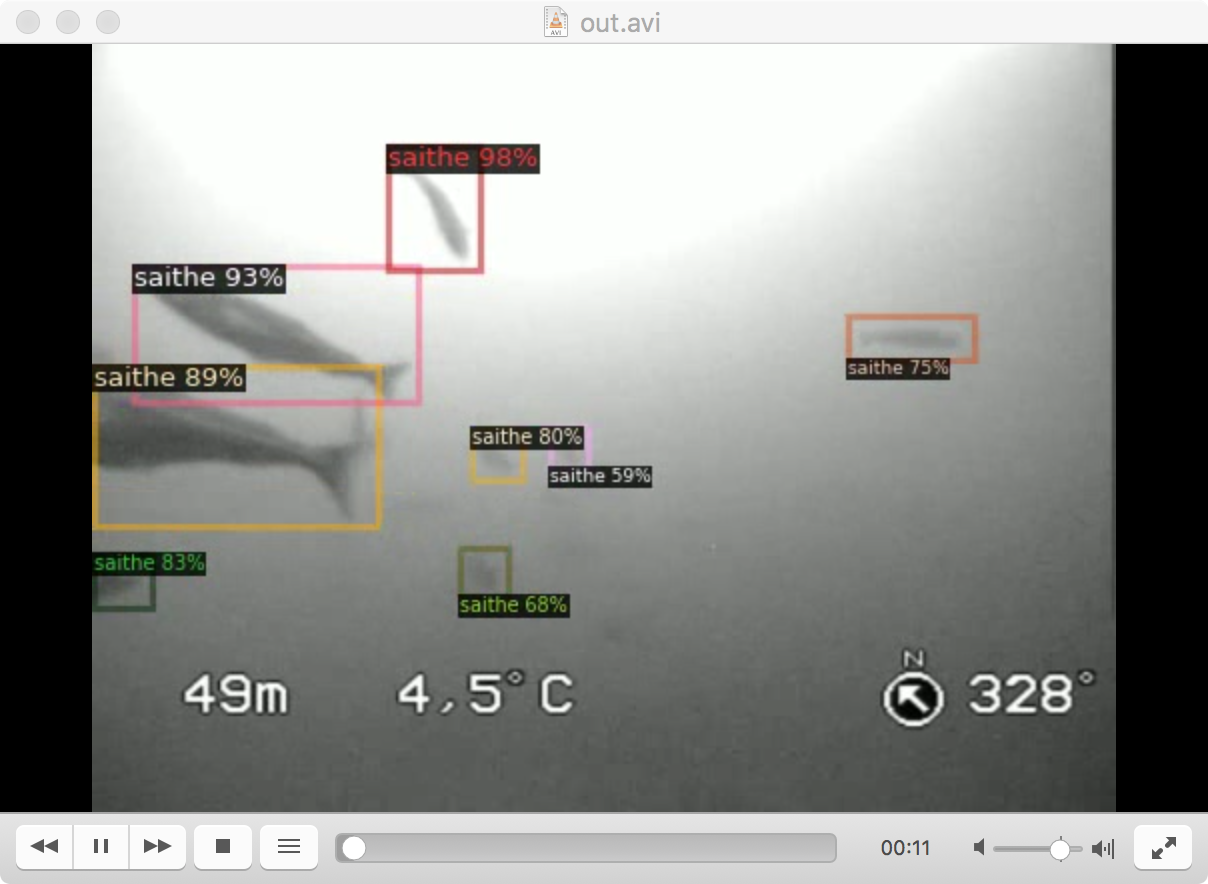
\includegraphics[scale=0.35]{figures/retinanet_inference_saithe}
\caption{\small \sl Sei RetinaNet. \label{fig:retinanet_inference_saithe}}
\end{center}
\end{figure}

Det ble trent opp to modeller, en RetinaNet modell og en YOLOv4 modell. Dataen av torsk bestod av tre kanaler, og hadde størrelsen 1920 $\times$ 1080. Bildene av sei bestod av kun en kanal, og hadde størrelsen 640 $\times$ 480. Dette fører til bias. Datasettet burde bestå av data uten bias. Modellene som er trent kan effektivt se forskjell på torsk og sei som finnes i bildene, men ettersom bildene ble tatt på så forskjellige måter, der sei dataen var i gråtoner og torsk var i farger, så vil modellen muligens se etter fisk av gråtoner, ikke sei, når den ser etter sei. Datasettet bestod av 208 bilder av torsk, med til sammen 4582 instanser av torsk i bildene. Det var 604 bilder av sei med 5525 instanser av fisken i bildene. Det er litt flere instanser av sei enn av torsk. Det kan også øke bias i modellen i noe grad.

Det som er lettere for mennesker å forstå er også lettere for maskiner å forstå. Data is king innenfor maskinsyn, å ha gode bilder er et must for å få gode resultater. Det betyr ikke at et bilde av gråtoner, eller av lav oppløsning er dårlige. Det er faktisk mange fordeler med gråtoner og lav oppløsning. De kan prosesseres raskt, og av og til så blir de viktigste egenskapene mer synlige.

A classification accuracy of 94.3 \% was achieved when classifying only the 16 fish species which we focussed on for this trial. All other evaluations include the other species class which contains a number of fish species which are non-relevant to the research goals, but can be encountered while underwater sampling. The re- sults obtained by the different model configurations are summa- rized in Table 2. The model based on ResNet (He et al., 2016) by cross-pooling activations from layer 4b15 and 4b20, with local region size of 3 and training of a linear SVM on top of the cross-pooled features, was able to achieve the highest classifica- tion accuracy of 89.0 \% if the other species class is included. A change to a local region size of 1 produces a slightly inferior result of 86.9 \% classification accuracy for all classes. In compari- son, the AlexNet and VGGNet model configurations produced significantly degraded results.

Application of the linear SVM di- rectly to features from the Pool5 layer of the ResNet-152 model resulted in a classification accuracy of 71.49 \%, highlighting the improved performance produced by cross-layer pooling. We re- duced the dimensionality of the 3 local features in ResNet- 152b model from 9216 (3 3 1024) to 512 before cross-layer pooling using PCA. Dimensionality reduction can be useful in or- der to reduce the size of features from cross-layer pooling, allow- ing use of larger region sizes as well as more feature maps. Adapting a larger region size even with the use of PCA improved accuracy of the system due to availability of local context. 

Further analysis of the accuracy of the four CNN models can be con- ducted using the precision and recall of the classifier. Recall and precision are a more informative way to judge the performance of a classifier, especially if the classes are skewed.

The precision of a classifier is a measure of correctly classified images out of all the images predicted to belong to a specific class. Mathematically,

\begin{equation}
\text{Precision} = \frac{\text{True positives}}{\text{True positives} + \text{False positives}}
\end{equation}

Recall of a classifier on the other hand is a measure of correctly classified images out of all the images actually belonging to a spe- cific class. Mathematically:

\begin{equation}
\text{Recall} = \frac{\text{True positives}}{\text{True positives} + \text{False negatives}}
\end{equation}

In general, the precision and recall graphs confirm the classifi- cation accuracy levels shown in Table 2, with very few exceptions. In some cases, the ResNet-152 model with a 1 1 local region produces the best result, but these exceptions reflect the small dif- ference in the classification accuracy between the two sizes of lo- cal region. Precision is generally higher than recall, indicating that false negatives are more common than false positives. The precision graph shows high values for a number of individual species, indicating that the number of false positives is very low. The lesser precision in ...

\subsection{RetinaNet}

\begin{figure}[h!]
\begin{center} 
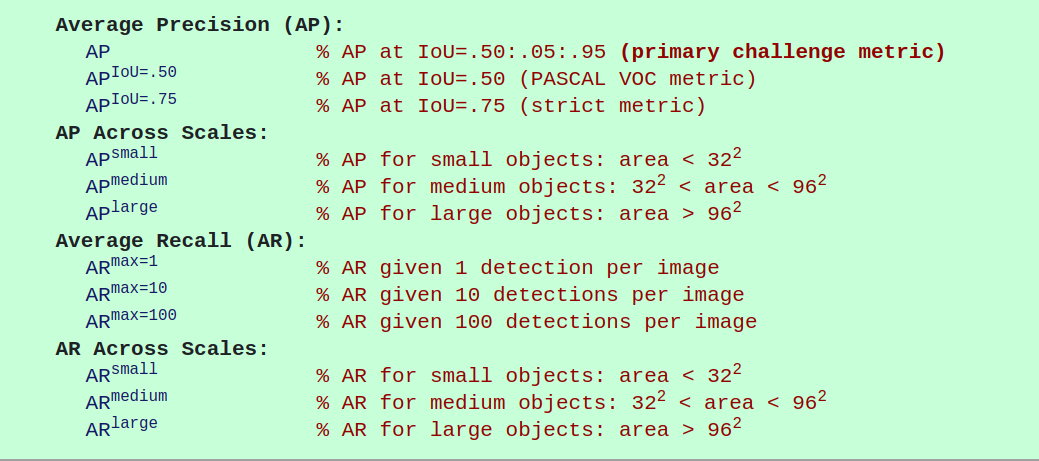
\includegraphics[scale=0.35]{figures/coco}
\caption{\small \sl You have to evaluate your detection model on COCO detection evaluation metric. For your reference here is the coco evaluation metric chart. \label{fig:coco}}
\end{center}
\end{figure}

The expected AP (primary challenge metric) is more than 0.5. \\
Output following: \\
 \\
 Average Precision  (AP) @[ IoU=0.50:0.95 | area=   all | maxDets=100 ] = 0.285 \\
 Average Precision  (AP) @[ IoU=0.50      | area=   all | maxDets=100 ] = 0.663 \\
 Average Precision  (AP) @[ IoU=0.75      | area=   all | maxDets=100 ] = 0.200 \\
 Average Precision  (AP) @[ IoU=0.50:0.95 | area= small | maxDets=100 ] = 0.067 \\
 Average Precision  (AP) @[ IoU=0.50:0.95 | area=medium | maxDets=100 ] = 0.217 \\
 Average Precision  (AP) @[ IoU=0.50:0.95 | area= large | maxDets=100 ] = 0.402 \\
 Average Recall     (AR) @[ IoU=0.50:0.95 | area=   all | maxDets=  1 ] = 0.038 \\
 Average Recall     (AR) @[ IoU=0.50:0.95 | area=   all | maxDets= 10 ] = 0.248 \\
 Average Recall     (AR) @[ IoU=0.50:0.95 | area=   all | maxDets=100 ] = 0.433 \\
 Average Recall     (AR) @[ IoU=0.50:0.95 | area= small | maxDets=100 ] = 0.139 \\
 Average Recall     (AR) @[ IoU=0.50:0.95 | area=medium | maxDets=100 ] = 0.352 \\
 Average Recall     (AR) @[ IoU=0.50:0.95 | area= large | maxDets=100 ] = 0.556 \\
Evaluation results for bbox:  \\
|   AP   |  AP50  |  AP75  |  APs  |  APm   |  APl   | \\
|:------:|:------:|:------:|:-----:|:------:|:------:| \\
| 28.494 | 66.262 | 20.016 | 6.654 | 21.663 | 40.239 | \\
Per-category bbox AP:  \\
| category     | AP     | category   | AP     | \\
|:-------------|:-------|:-----------|:-------| \\
| atlantic\_cod | 23.077 | saithe     | 33.910 |

\begin{figure}[h!]
\begin{center} 
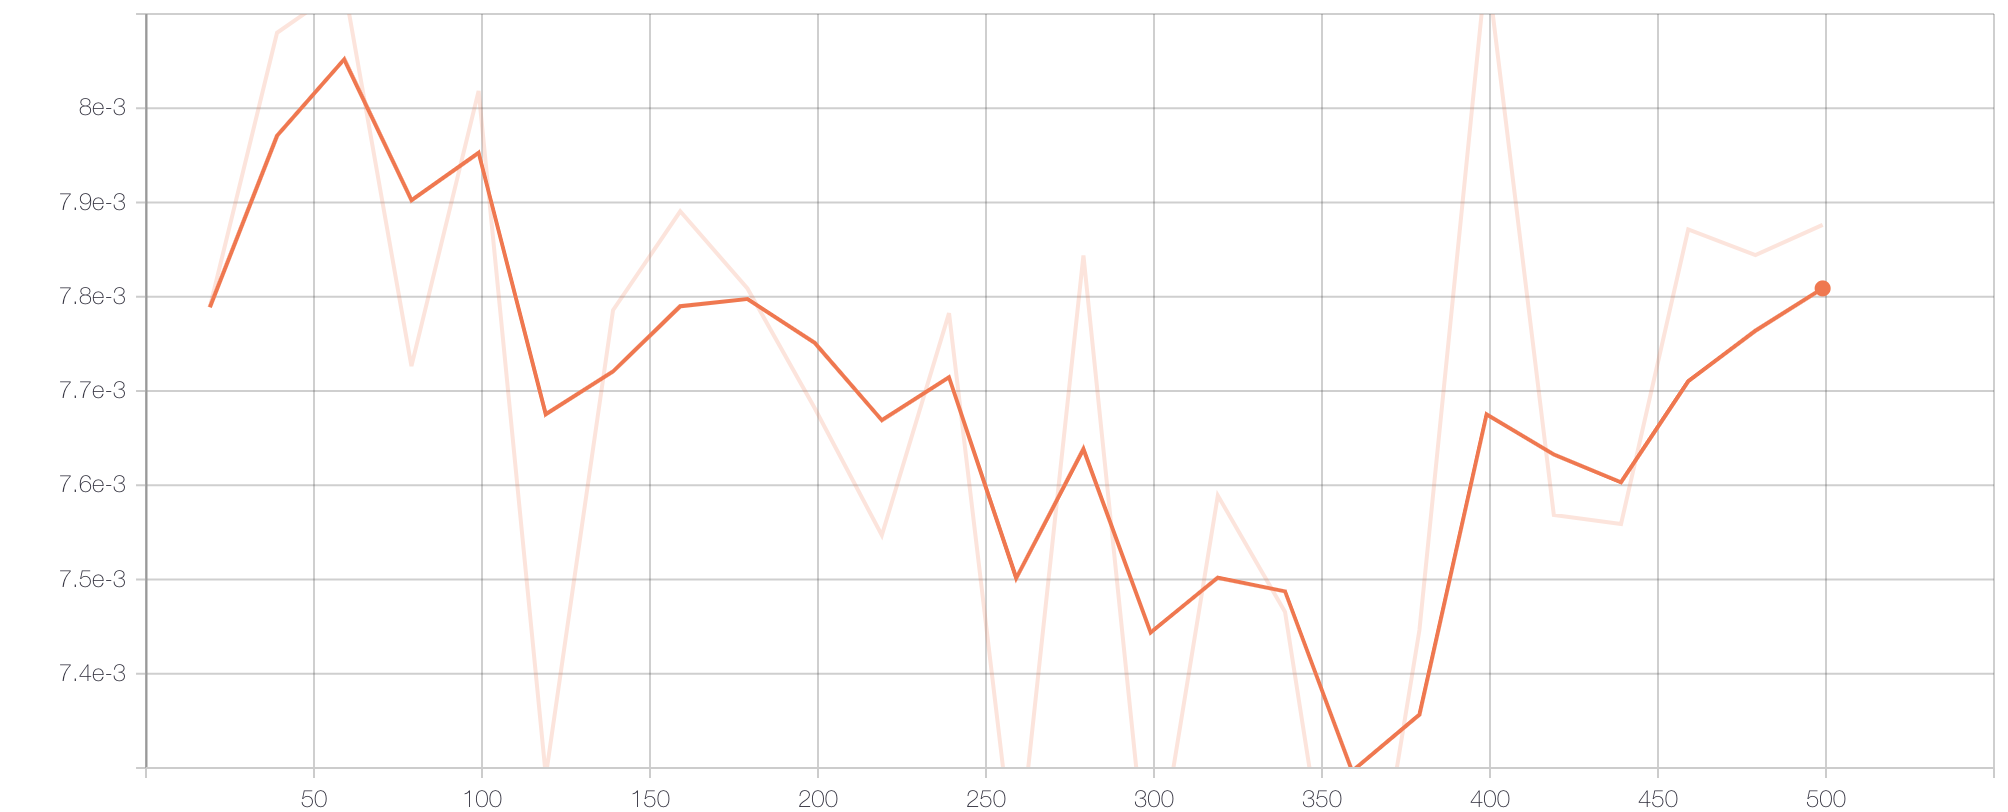
\includegraphics[scale=0.35]{figures/data_time_retinanet_1}
\caption{\small \sl data time RetinaNet. \label{fig:data_time_retinanet}}
\end{center}
\end{figure}

\begin{figure}[h!]
\begin{center} 
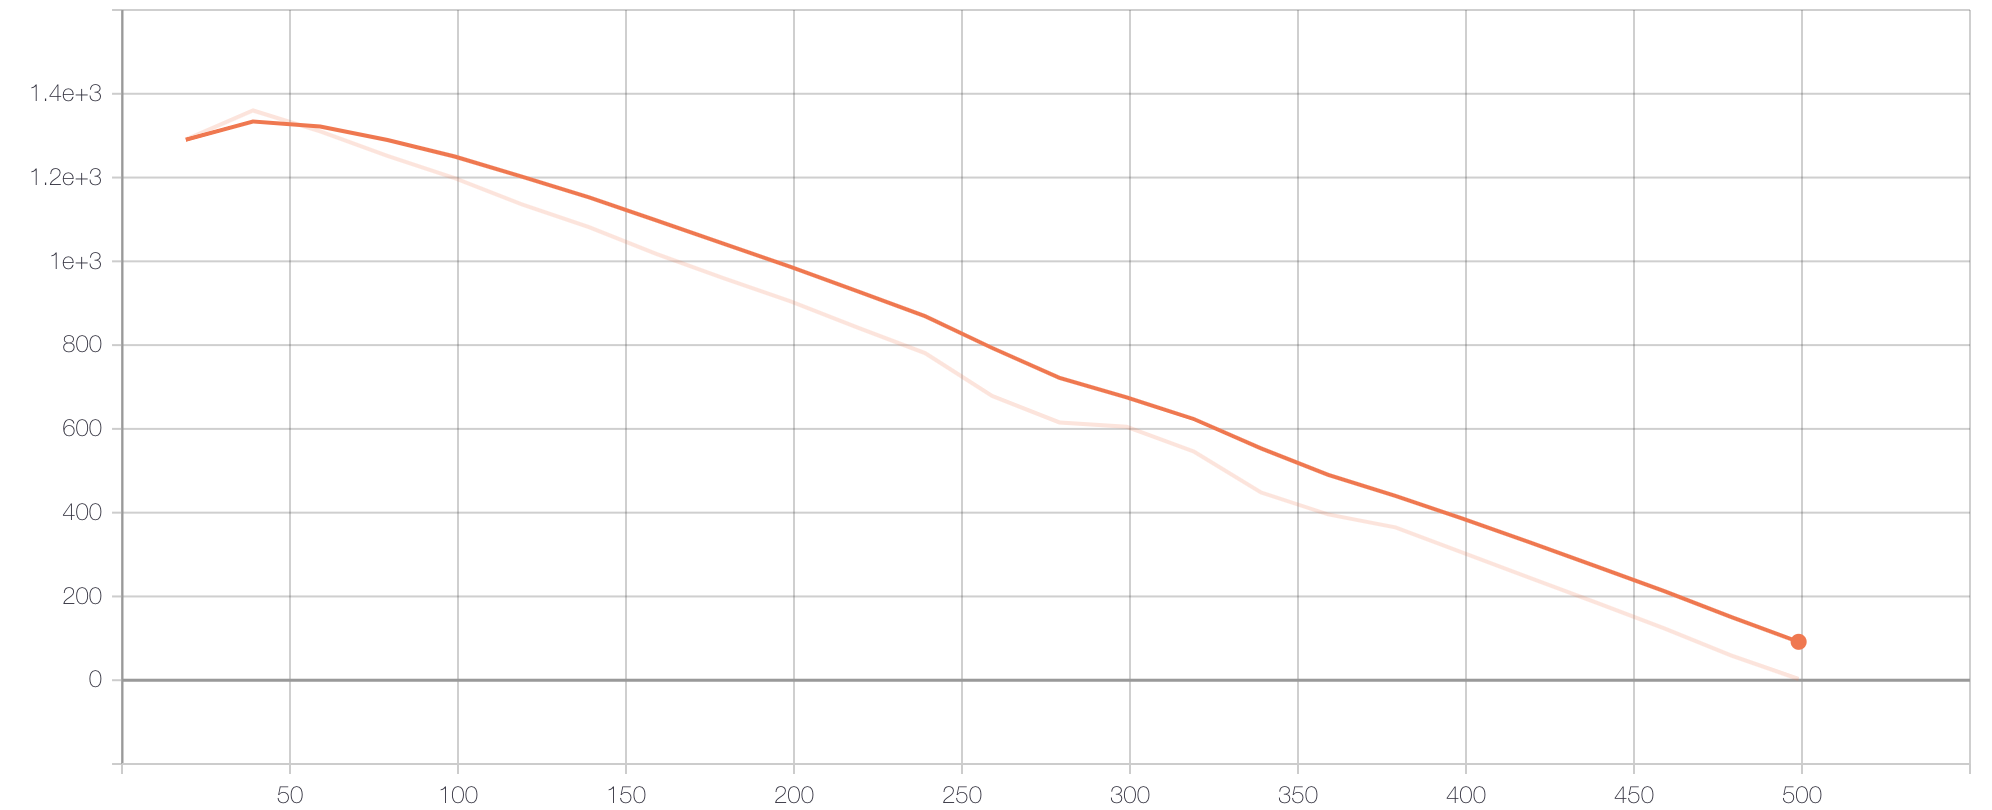
\includegraphics[scale=0.35]{figures/eta_seconds_retinanet_2}
\caption{\small \sl eta seconds RetinaNet. \label{fig:eta_seconds_retinanet}}
\end{center}
\end{figure}

\begin{figure}[h!]
\begin{center} 
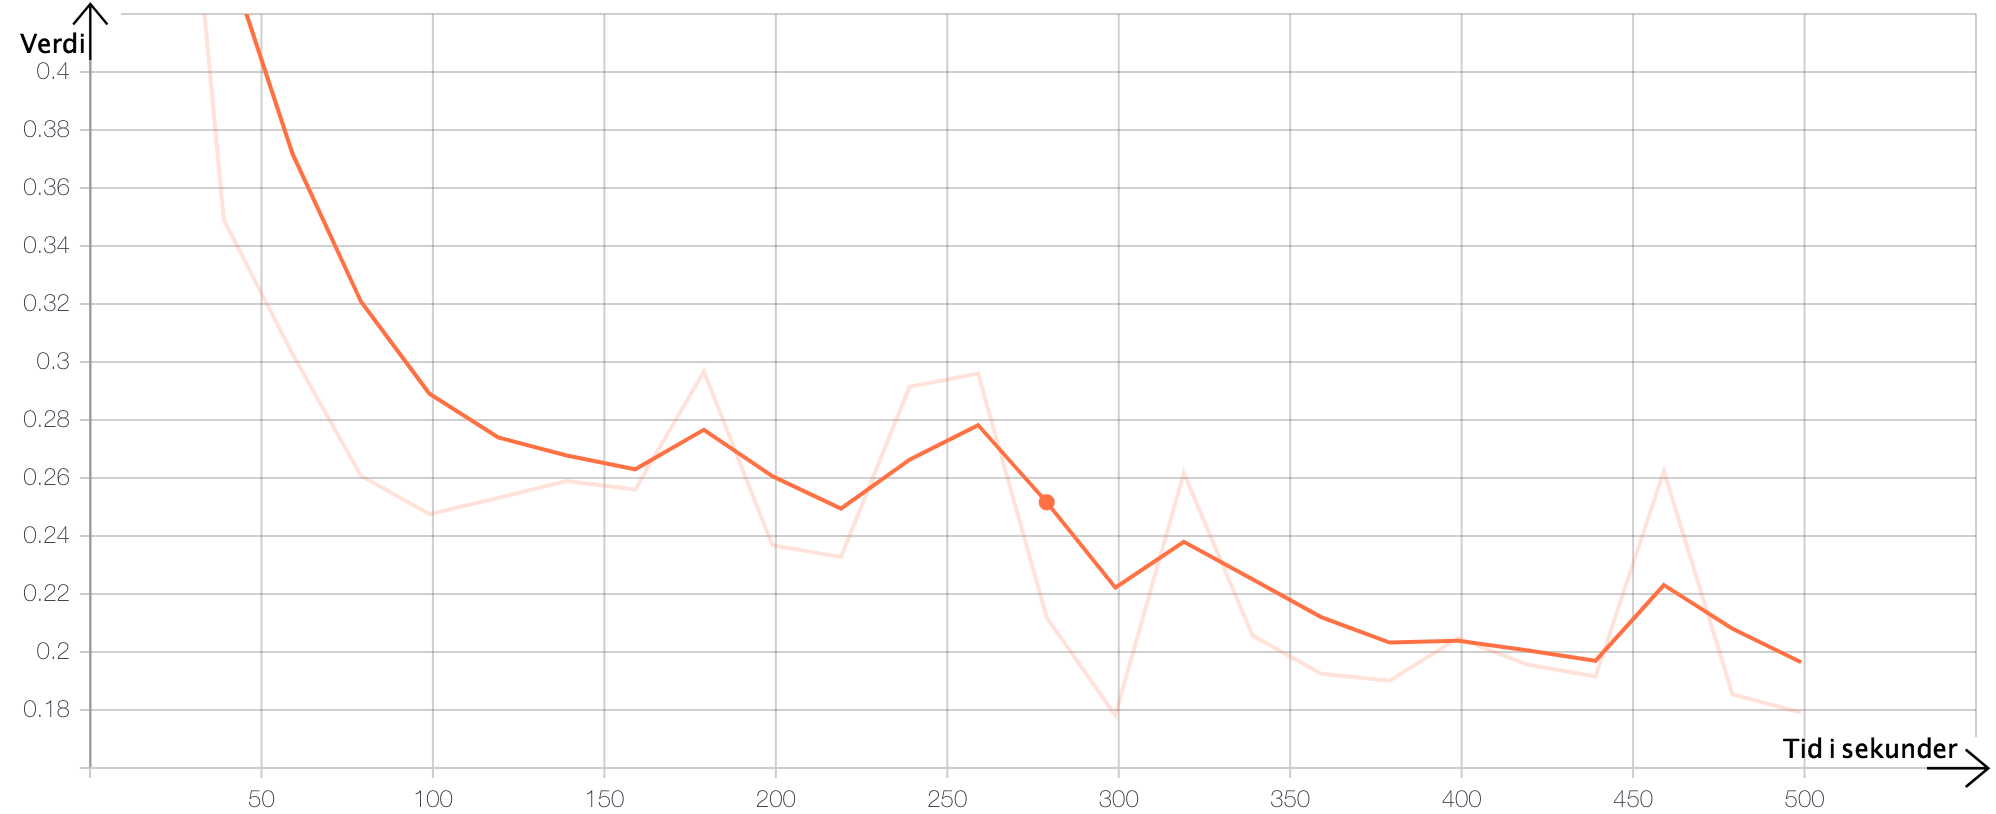
\includegraphics[scale=0.35]{figures/loss_box_reg_retinanet_3}
\caption{\small \sl loss box reg RetinaNet. \label{fig:loss_box_reg_retinanet}}
\end{center}
\end{figure}

\begin{figure}[h!]
\begin{center} 
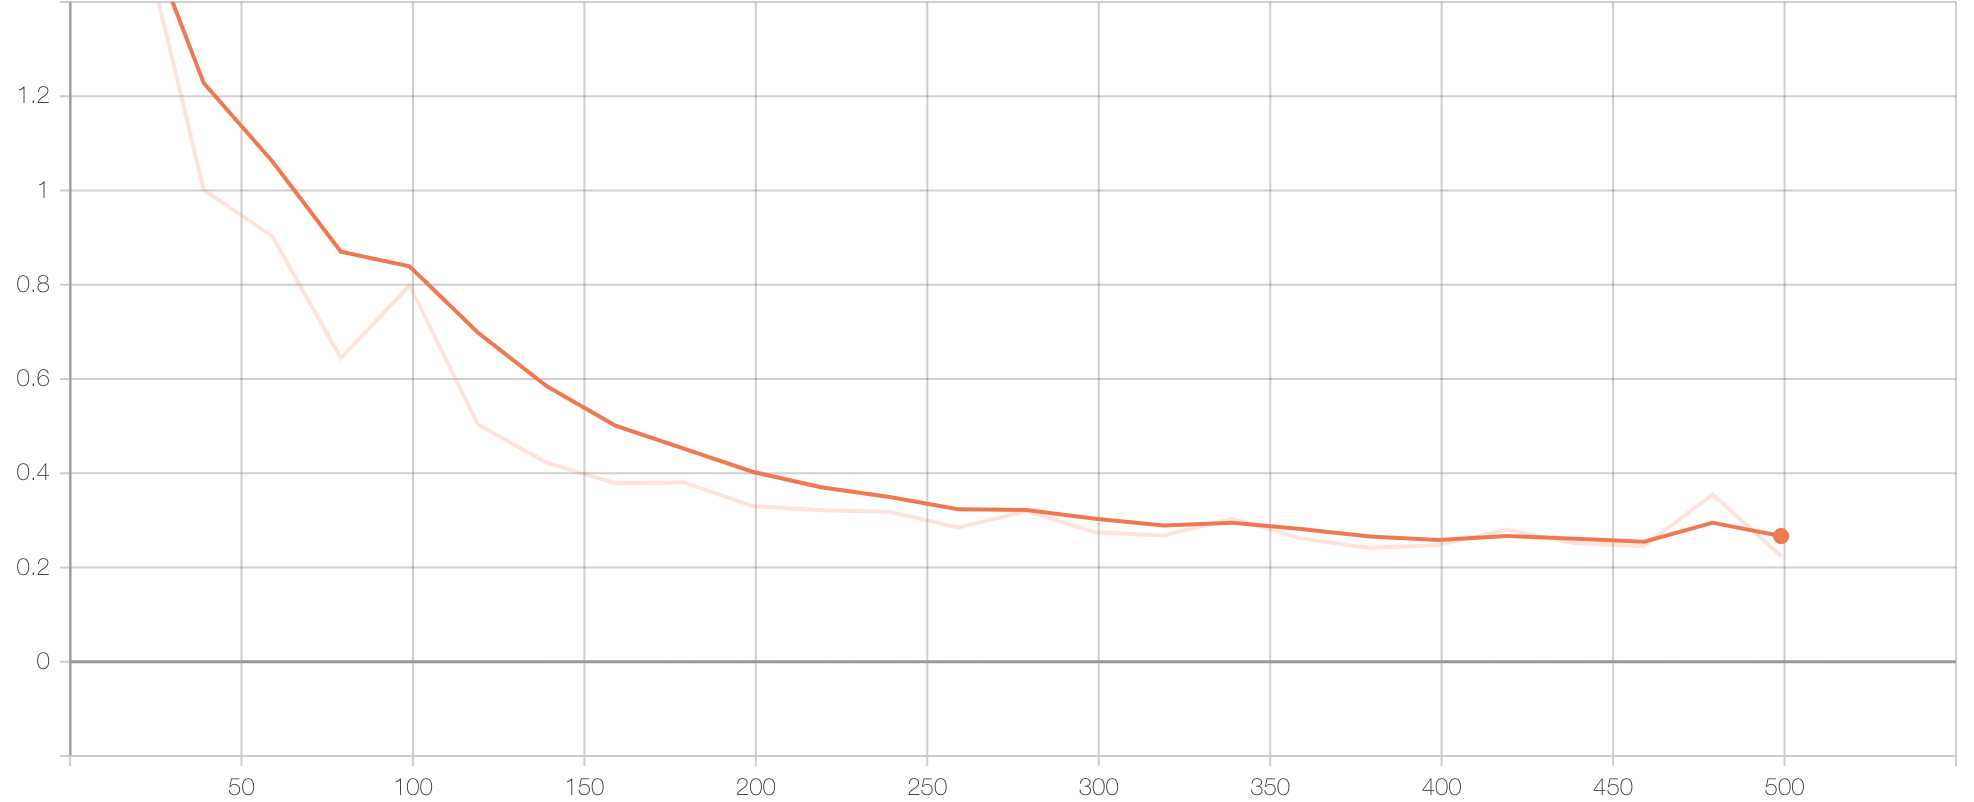
\includegraphics[scale=0.35]{figures/loss_cls_retinanet_4}
\caption{\small \sl loss cls RetinaNet. \label{fig:loss_cls_retinanet}}
\end{center}
\end{figure}

\begin{figure}[h!]
\begin{center} 
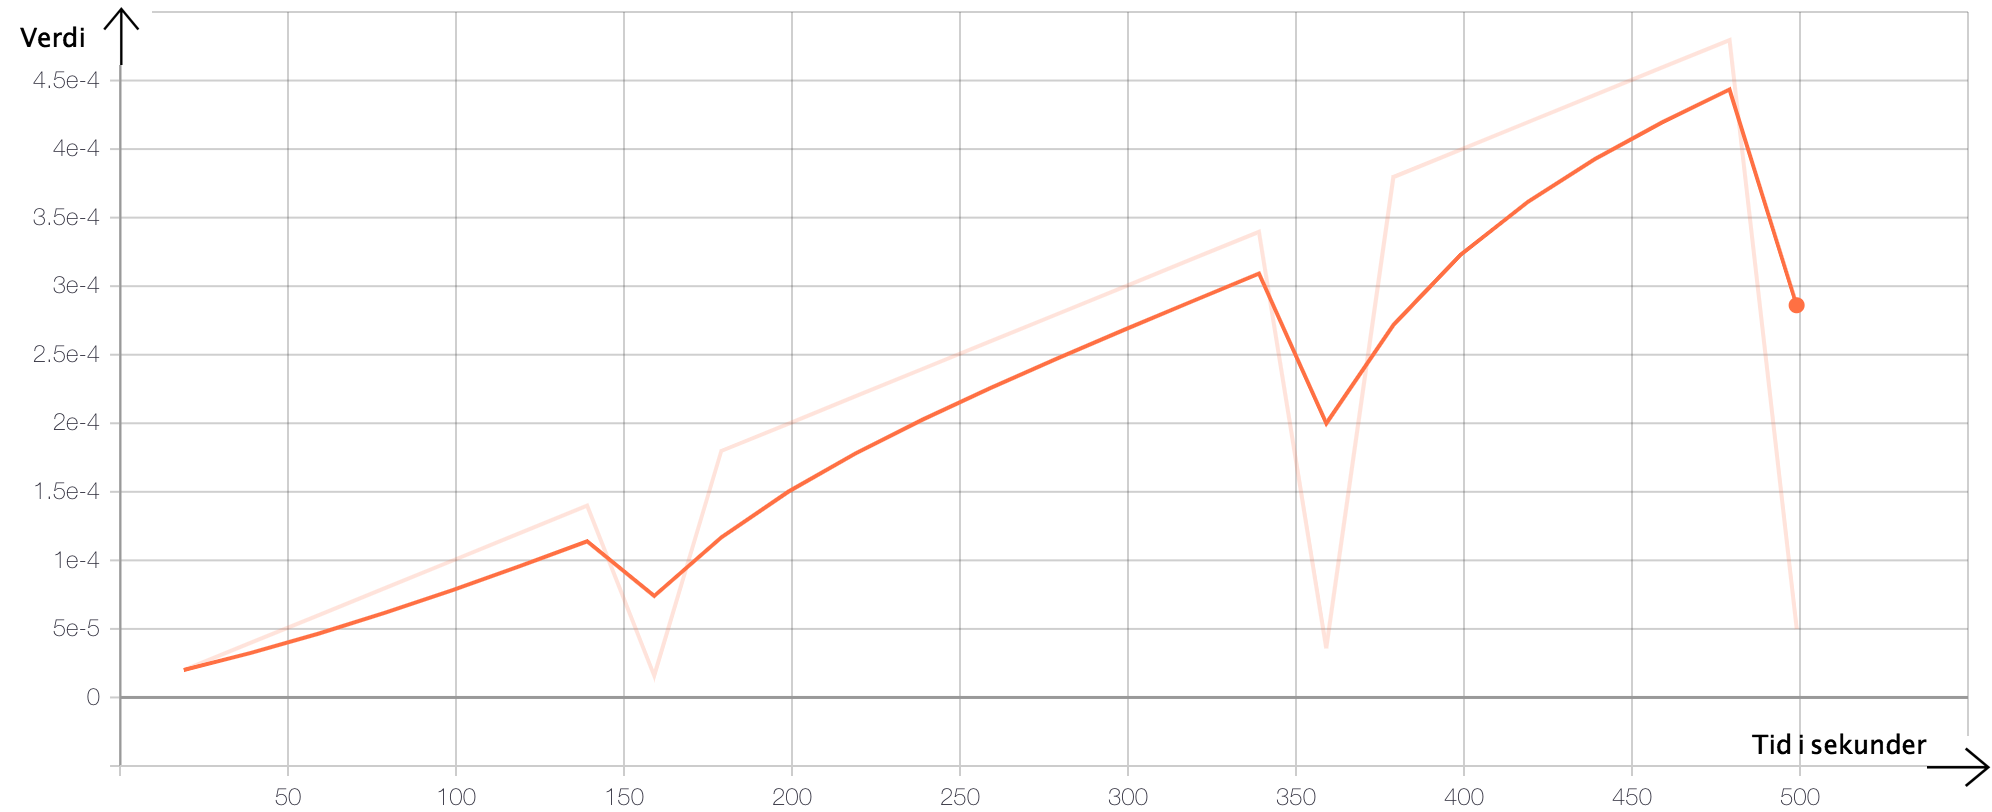
\includegraphics[scale=0.35]{figures/lr_retinanet_5}
\caption{\small \sl learning rate RetinaNet. \label{fig:lr_retinanet}}
\end{center}
\end{figure}

\begin{figure}[h!]
\begin{center} 
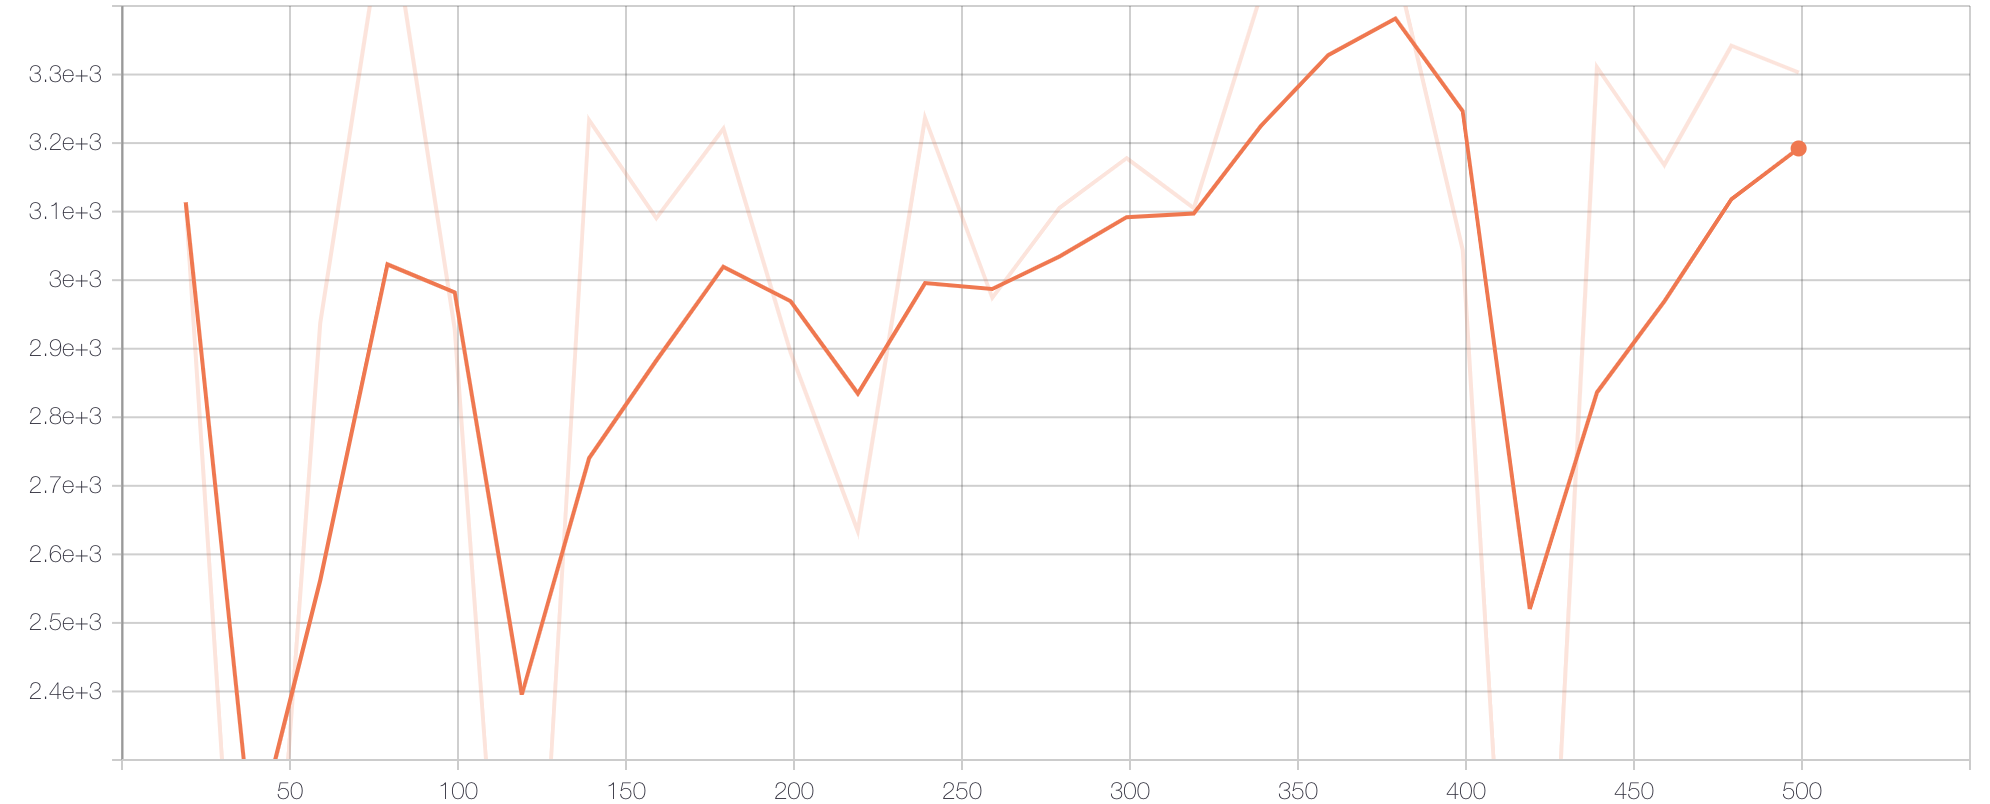
\includegraphics[scale=0.35]{figures/num_foreground_6}
\caption{\small \sl num foreground RetinaNet. \label{fig:num_foreground}}
\end{center}
\end{figure}

\begin{figure}[h!]
\begin{center} 
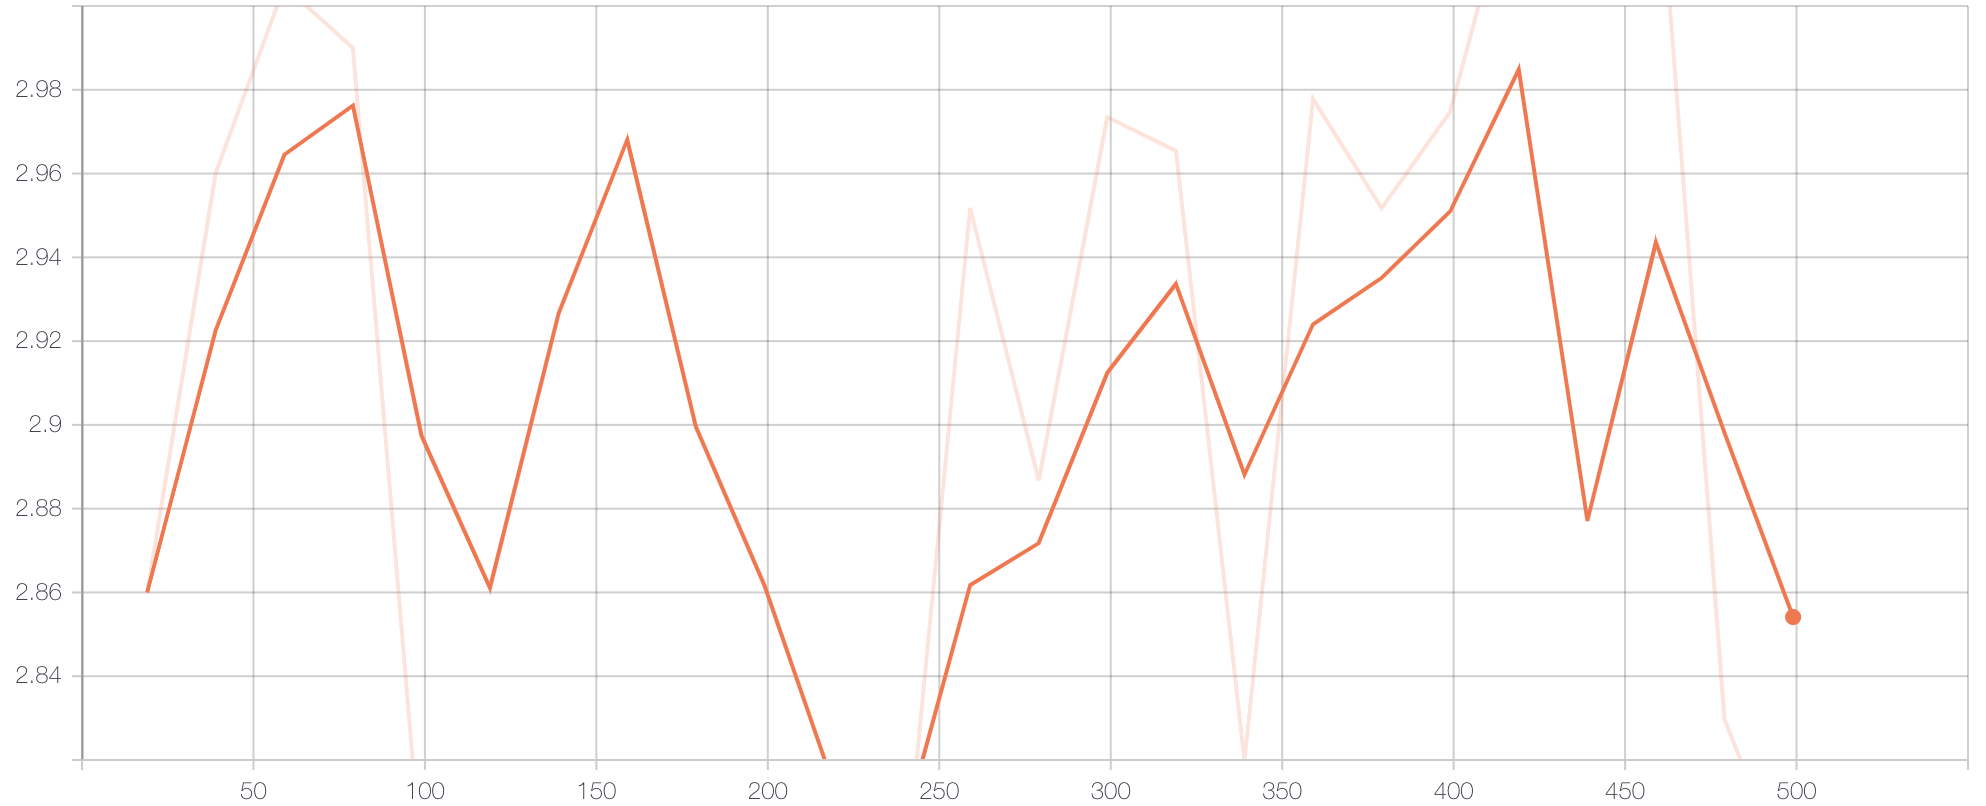
\includegraphics[scale=0.35]{figures/time_retinanet_7}
\caption{\small \sl time RetinaNet. \label{fig:time_retinanet}}
\end{center}
\end{figure}

\begin{figure}[h!]
\begin{center} 
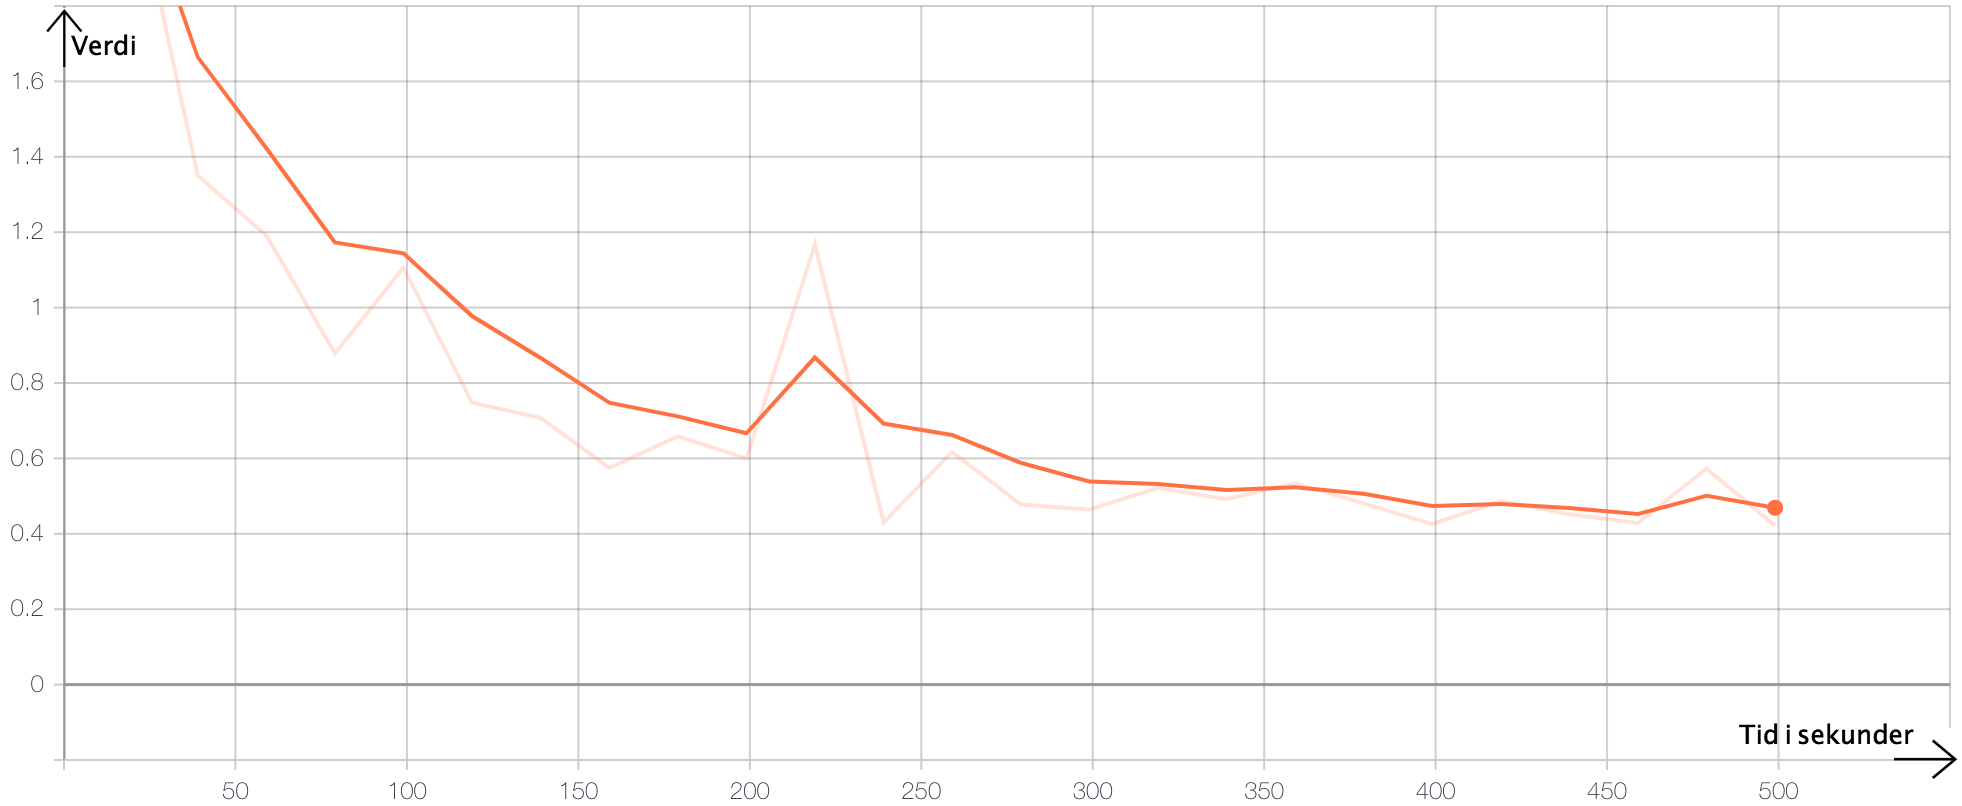
\includegraphics[scale=0.35]{figures/total_loss_retinanet_8}
\caption{\small \sl total loss RetinaNet. \label{fig:total_loss_retinanet}}
\end{center}
\end{figure}

RetinaNet resultatene for dette eksperimentet er også tilgjengelige på nettet. Se \\ \url{https://tensorboard.dev/experiment/2PxmdvA5QdavQC0YLABdgw}.

\subsubsection{COCO deteksjonsevaluering} 

\subsection{YOLO}

\begin{figure}[h!]
\begin{center} 
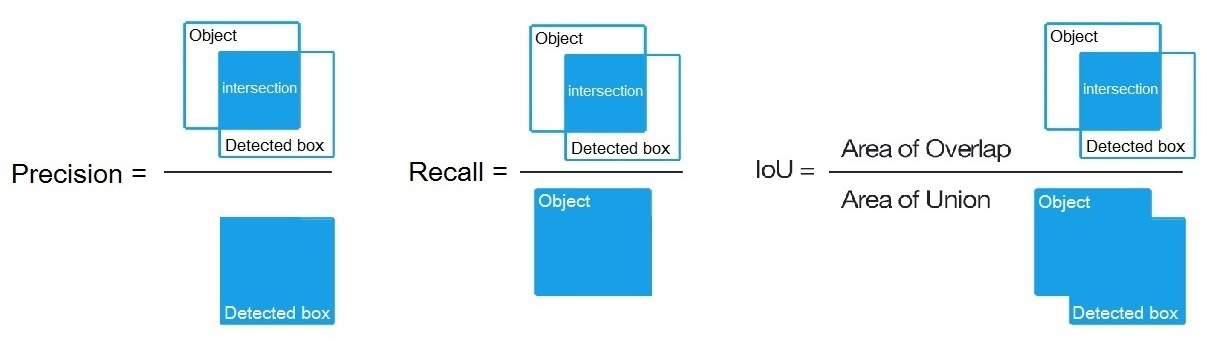
\includegraphics[scale=0.45]{figures/precision}
\caption{\small \sl Precision, recall og IoU. \cite{Bochkovskiy 2020} \label{fig:precision}}
\end{center}
\end{figure}

IoU (intersect over union) - average instersect over union of objects and detections for a certain threshold = 0.24

mAP (mean average precision) - mean value of average precisions for each class, where average precision is average value of 11 points on PR-curve for each possible threshold (each probability of detection) for the same class (Precision-Recall in terms of PascalVOC, where Precision=TP/(TP+FP) and Recall=TP/(TP+FN) ), %page-11: http://homepages.inf.ed.ac.uk/ckiw/postscript/ijcv_voc09.pdf

mAP is default metric of precision in the PascalVOC competition, this is the same as AP50 metric in the MS COCO competition. In terms of Wiki, indicators Precision and Recall have a slightly different meaning than in the PascalVOC competition, but IoU always has the same meaning.

\begin{figure}[h!]
\begin{center} 
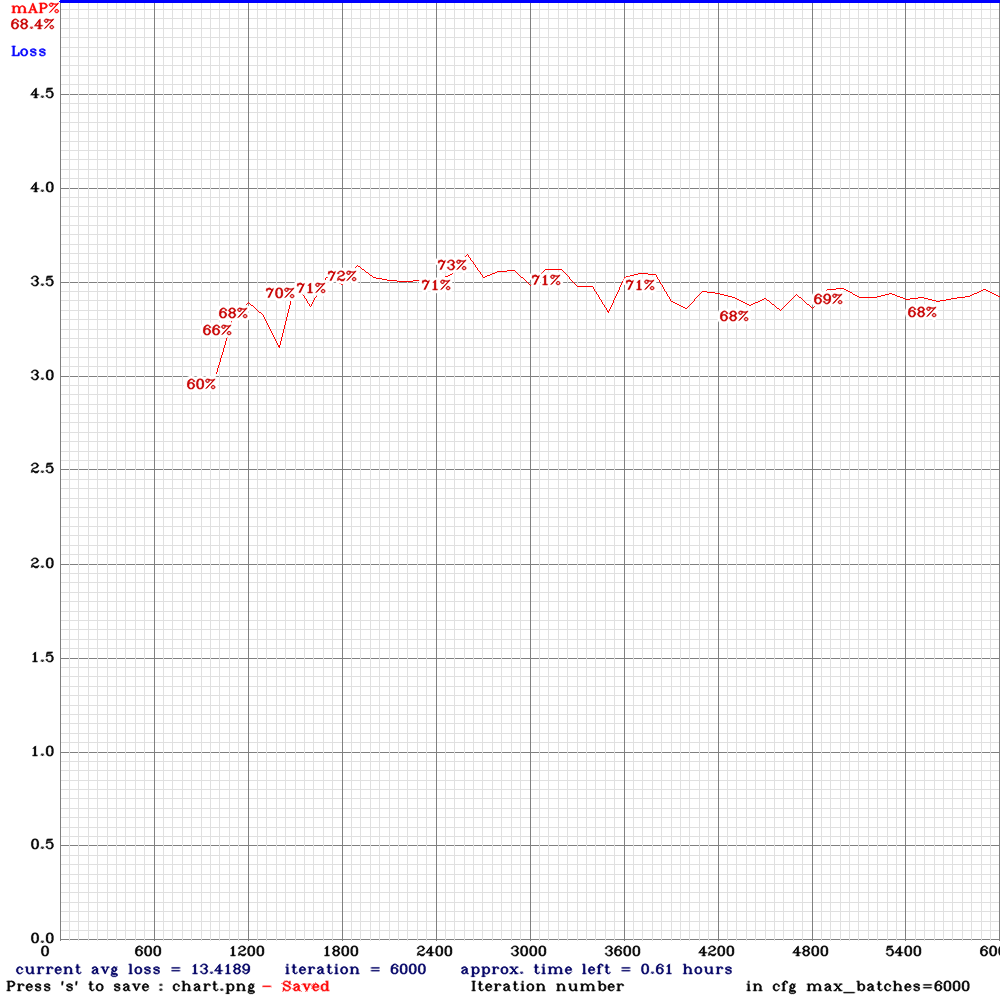
\includegraphics[scale=0.35]{figures/chart_yolo-obj.png}
\caption{\small \sl graf YOLO. \label{fig:chart_yolo}}
\end{center}
\end{figure}